\chapter{Rotation of the Hand UI Model}

\label{Chapter4_rotation} 

\begin{comment}
-------------------------------------------------
%								Chapter layout
4. Rotation of Hand UI Model
	a. Description of Problem
	a. JavaFx Coordinate System vs Leap Motion Coordinate System
	b. Ineffective Leap Motion Data
		i. Pitch Roll Yaw
		ii. Negative Zeros
	c. Simplified Hand Model
	d. Composite Linear Transformations
	e. Rotational Matrix
-------------------------------------------------
\end{comment}
In this chapter the rotation of the Hand UI model will be discussed. 

%------------------------------------------------
%	SECTION 1 Description of Problem
%------------------------------------------------
\section{Description of Problem}
The UI model of the hand is built from the Leap Motion sensor data as discussed in the chapter. This data represents the hand as it is displayed in reality above the Leap Motion controller device. Originally the representation of the hand was built from this hand without any further modifications. However, to demonstrate why this is sometimes not the ideal situation, see Figure \ref{fig:handFlat}. It shows the hand as it is displayed in reality; it is in parallel plane above the device. 
\begin{figure}[H]
\centering
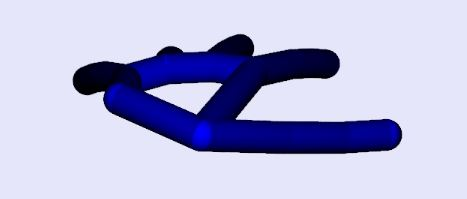
\includegraphics[scale=0.45]{Figures/4_handFlat.JPG}
\caption[Hand in Flat Orientation]{This shows the user's hand in a flat orientation; as determined by the Leap Motion sensor.}
\label{fig:handFlat}
\end{figure}
It should noted how difficult it is to see the fingers and thumb. They are only barely visible. Therefore the user would be forced to force his or her hand into a vertical postion by straining their wrist just so they can see the gesture they are performing on the screen. Figures \ref{fig:handYaw} and \ref{fig:handRoll} show other orientation the hand can take; these figures show the hand after a yaw rotation and after a roll rotation respectively. Again, note the slight difficulty in figuring out the thumb and fingers positions and orientations when the hand is rolled around the z-axis. The hand that is shown in the yaw rotation in Figure \ref{fig:handYaw} is able to seen a little clearly because the wrist was strained upwards. 
\begin{figure}[H]
    \centering
    \begin{minipage}{0.5\textwidth}
        \centering
        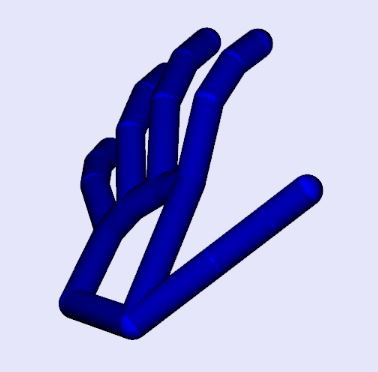
\includegraphics[scale=.55]{Figures/4_handYaw.JPG} 
        \caption[Hand with Yaw Rotation]{The user's hand after the certain yaw rotation around the y-axis.}
		\label{fig:handYaw}
    \end{minipage}\hfill
    \begin{minipage}{0.5\textwidth}
        \centering
        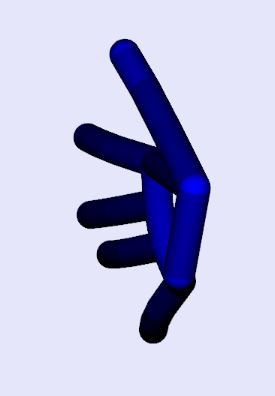
\includegraphics[scale=.55]{Figures/4_handRoll.JPG}
        \caption[Hand with Roll Rotation]{The user's hand after the certain roll rotation around the z-axis.}
        \label{fig:handRoll}
    \end{minipage}
\end{figure}
Finally all of these different orientation can of course overlap with each other to create a complex orientation of the hand as shown in Figure \ref{fig:weirdHandShake}, which shows the user's left hand in a weird handshake sort of position while being rotated to the right and tilted upwards.
\begin{figure}[H]
\centering
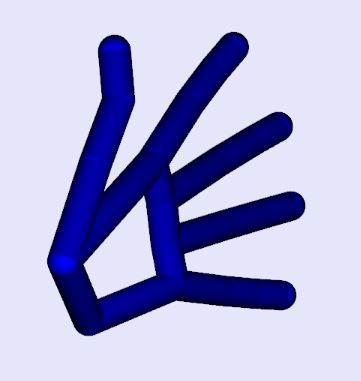
\includegraphics[scale=0.45]{Figures/4_handWeirdHandshake.JPG}
\caption[Hand in Weird Handshake Position]{This shows the user's hand in a flat orientation; as determined by the Leap Motion sensor.}
\label{fig:weirdHandShake}
\end{figure}
This chapter will explain how these different possible orientations the user's hand might be in while they are performing gestures shown on the screen are accounted for and "undone". Doing this results in the user's hand to be displayed in a set vertical orientation on the screen despite the different ways the user may have oriented their hand above the device in reality. The final resulting hand for all of the figures seen previously  will be as is shown in Figure \ref{fig:handFinalResult} after the composite rotation have transformed it to a vertical position. 
\begin{figure}[H]
\centering
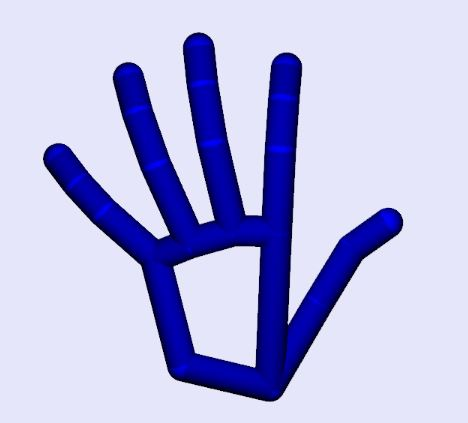
\includegraphics[scale=0.45]{Figures/4_handFinalFix.JPG}
\caption[Hand Fixed to Vertical Orientation]{This shows what the user's hand will look like after all of the possible rotational transforms have been undone and the hand has been fixed to a vertical orientation.}
\label{fig:weirdHandShake}
\end{figure}
This feature of the application makes it easier for the user to see what his or her hand is doing without requiring them to always contain their hand in a specific orientation. The goal of this application is to measure the accuracy with which a user is able to complete certain gestures, not the orientation of their hand. In fact, the algorithms that are used to grade the correctness of the user's attempted gesture do not take the user's hand orientation into account. They focus on the fingers bones and their relative orientations to each other. At the beginning of this project, one of the ideas discussed was to build some sort of rig which would be used to place the user's hand in a set orientation. However because of what will be explained in this chapter such a rig is no longer necessary.



%------------------------------------------------
%	SECTION 1 JavaFx CS vs Leap Motion CS
%------------------------------------------------

\section{JavaFx Coordinate System vs Leap Motion Coordinate System}
	


%------------------------------------------------
%	SECTION 2 Ineffective Leap Motion Data
%------------------------------------------------
\section{Ineffective Leap Motion Data}


%----------------------------------- Pitch Roll Yaw
\subsection{Pitch Roll Yaw}


%----------------------------------- Negative Zeros
\subsection{Negative Zeros}




%------------------------------------------------
%	SECTION 3 Simplified Hand Model
%------------------------------------------------

\section{Simplified Hand Model}
	
	
%------------------------------------------------
%	SECTION 4 Composite Linear Transformations
%------------------------------------------------

\section{Composite Linear Transformations}





%------------------------------------------------
%	SECTION 5 Rotational Matrix
%------------------------------------------------

\section{Rotational Matrix}





